\section{Leistungsfluss über eine Leitung}

\subsubsection{Mathematische Vereinfachungen im Voraus}

\begin{minipage}[c]{0.48\columnwidth}
        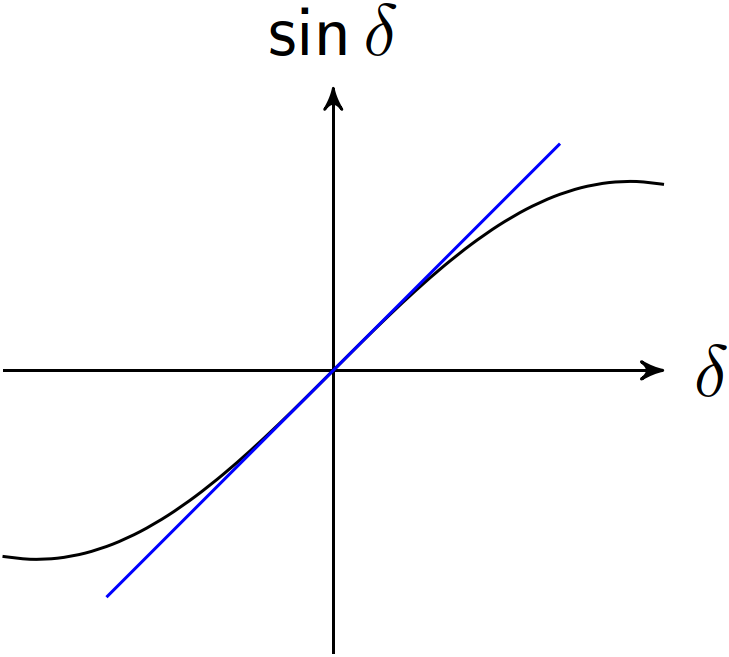
\includegraphics[width=0.7\textwidth, align=c]{images/Erkenntnisse_1.png}
\end{minipage}
\hfill
\begin{minipage}[c]{0.48\columnwidth}
        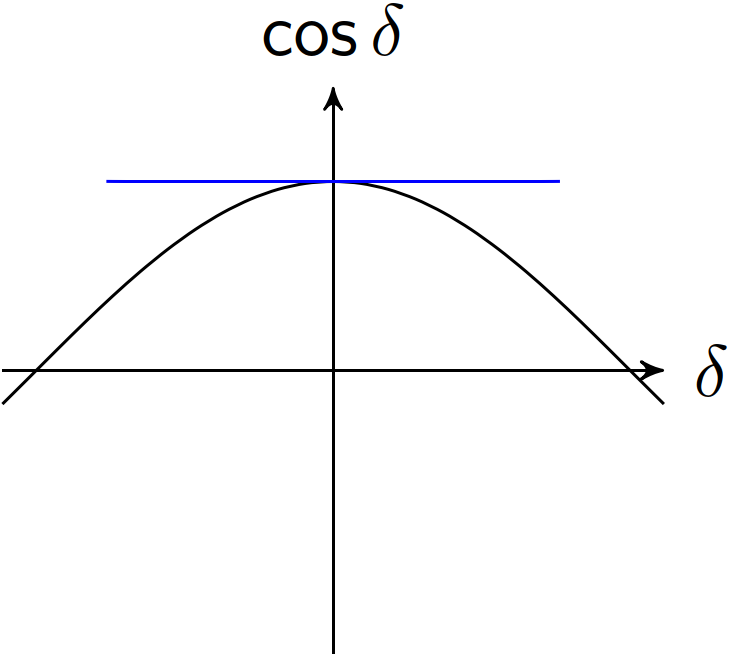
\includegraphics[width=0.7\textwidth, align=c]{images/Erkenntnisse_2.png}
\end{minipage}

\vspace{0.15cm}

\begin{minipage}[c]{0.48\columnwidth}
    \begin{itemize}
        \item für kleinere Winkel: $\sin\delta \approx \delta$
        \item Maximale Steigung
    \end{itemize}    
\end{minipage}
\hfill
\begin{minipage}[c]{0.48\columnwidth}
    \begin{itemize}
        \item für kleinere Winkel: $\cos\delta \approx 1$
        \item Minimale Steigung
    \end{itemize}
\end{minipage}


\subsection{Leistungsfluss}

\begin{itemize}
    \item Verlustlose Leitung
    \item Ideale Spannungsquellen $\underline{U}_1$ und $\underline{U}_2$
\end{itemize}

\vspace{0.15cm}

\includegraphics[width=0.75\columnwidth]{images/Leistungsübertragung_1.png}

\vspace{0.15cm}


\subsection{Leistungsübertragung}

$
\boxed{\underline{U}_1 = U_1 \cdot e^{j \cdot \theta_1}} \quad \boxed{\underline{U}_2 = U_2 \cdot e^{j \cdot \theta_2}}
$

\vspace{0.15cm}

$
\boxed{X_L = \omega \cdot L}
\quad
\boxed{X_L = \omega \cdot L' \cdot l}
\quad
\boxed{\omega = 2 \cdot \pi \cdot f}
$

\vspace{0.15cm}

$
\boxed{
\underline{I}_1 = \frac{U_1 - U_2}{j \cdot X_L} = \frac{U_1 \cdot e^{j \cdot \theta_1} - U_2 \cdot e^{j \cdot \theta_2}}{j \cdot X_L}} \quad 
$


$
\boxed{
\underline{I}_1^* = \frac{U_1 \cdot e^{-j \cdot \theta_1} - U_2 \cdot e^{-j \cdot \theta_2}}{-j \cdot X_L}
= \frac{j}{X_L} \left( U_1 \cdot e^{-j \cdot \theta_1} - U_2 \cdot e^{-j \cdot \theta_2} \right)
}
$

\vspace{0.15cm}

$\boxed{\delta = \theta_1 - \theta_2}$

\vspace{0.15cm}

$\boxed{\underline{S}_1 = \underline{U}_1 \cdot \underline{I}_1^*} \quad \boxed{\underline{S}_1 = {P}_1 + j \cdot {Q}_1} \quad  \quad $

$\boxed{
\underline{S}_1 = \underbrace{U_1 \cdot U_2 \cdot \frac{1}{X_L} \cdot \sin(\delta)}_{P_1}
+ j\, \underbrace{\left( U_1^2 \cdot \frac{1}{X_L} - U_1 \cdot U_2 \cdot \frac{1}{X_L} \cos(\delta) \right)}_{Q_1}}$

\vspace{0.15cm}

$
\boxed{P_1 = \text{Re}\{ \underline{U}_1 \cdot \underline{I}_1^*\}} \quad \boxed{P_1 = U_1 \cdot U_2 \cdot \frac{1}{X_L} \cdot \sin(\delta)}
$

\vspace{0.15cm}

$
\boxed{Q_1 = \text{Im}\{ \underline{U}_1 \cdot \underline{I}_1^*\}} \quad 
\boxed{Q_1 = U_1^2 \cdot \frac{1}{X_L} - U_1 \cdot U_2 \cdot \frac{1}{X_L} \cos(\delta)}
$

\vspace{0.15cm}

\renewcommand{\arraystretch}{1.2}
\begin{tabular}{@{} l p{6cm} l @{}}
$U_1$        & Effektive Spannungen am Leitungsanfang \dotfill & $\mathrm{V}$ \\
$U_2$        & Effektive Spannungen am Leitungsende \dotfill & $\mathrm{V}$ \\
$\theta_1$ & Phasenwinkel der Spannungen am Leitungsanfang \dotfill & $\mathrm{rad}$ \\
$\theta_2$ & Phasenwinkel der Spannungen am Leitungsende \dotfill & $\mathrm{rad}$ \\
$j$                 & Imaginäre Einheit ($j^2 = -1$) \dotfill & $-$ \\
$\omega$            & Kreisfrequenz \dotfill & $\mathrm{rad/s}$ \\
$f$                 & Netzfrequenz \dotfill & $\mathrm{Hz}$ \\
$L$                 & Induktivität der Leitung \dotfill & $\mathrm{H}$ \\
$L'$                & Induktivität pro Längeneinheit \dotfill & $\mathrm{H/m}$ \\
$l$                 & Leitungslänge \dotfill & $\mathrm{m}$ \\
$X_L$               & Reaktanz der Leitung  \dotfill & $\Omega$ \\
$I_1$               & Strom am Leitungsanfang \dotfill & $\mathrm{A}$ \\
$I_1^*$             & Komplex konjugierter Strom \dotfill & $\mathrm{A}$ \\
$S_1$               & Scheinleistung am Leitungsanfang \dotfill & $\mathrm{VA}$ \\
$P_1$               & Wirkleistung \dotfill & $\mathrm{W}$ \\
$Q_1$               & Blindleistung \dotfill & $\mathrm{VAR}$ \\
$\delta$           & Phasendifferenz \dotfill & $\mathrm{rad}$ \\
\end{tabular}

\newcolumn
\subsection{Praxis (Vereinfachung)}

\begin{itemize}
    \item $U_1 \approx U_2$
    \item $\delta$ in der Regel klein, $\delta \leq 40^\circ$
\end{itemize}

\vspace{0.15cm}
Mit den Vereinfachungen (Anfangs Kapitel) und den aufgeführten Punkten ergibt sich:
\vspace{0.15cm}

$\boxed{P_1 = U_1 \cdot U_2 \cdot \frac{1}{X_L} \cdot \delta}$ 

$\boxed{Q_1 = U_1 \cdot \frac{1}{X_L} \cdot (U_1 - U_2)}$ 

\vspace{0.15cm}


\subsubsection{Erkenntisse für Wirk- und Blindleistung}

\begin{itemize}
    \item \textbf{Wirkleistung}
    \begin{itemize}
        \item Stark abhängig von der Spannungswinkeldifferenz $\delta$
        \item wenig abhängig von der Spannungsbetrag $U_1, U_2$
    \end{itemize}
    
    \item \textbf{Blindleistung}
    \begin{itemize}
        \item wenig von der Spannungswinkeldifferenz $\delta$
        \item Stark abhängig von der Spannungsbetragsdifferenz $U_1 - U_2$
    \end{itemize}
\end{itemize}




\subsection{Maximale Wirkleistungsübertragung}

\begin{minipage}[c]{0.48\columnwidth}
    \includegraphics[width=0.7\textwidth, align=c]{images/Maximale_Wirkleistungsübertragung.png}
\end{minipage}
\hfill
\begin{minipage}[c]{0.48\columnwidth}
    $
    \boxed{P_{1_{\text{max}}} = \frac{U_1 \cdot U_2}{X_L}}
    $
\end{minipage}




